% {{{
\documentclass[a4paper,10pt,norsk]{article}
\usepackage[utf8]{inputenc}
\usepackage[english]{babel}
\usepackage{graphicx, verbatim, amsmath, amsfonts, geometry, float, import, bm}
\usepackage{siunitx} % converts expression to SI units/notation , \num{10e-10}
\usepackage[hidelinks]{hyperref}
\usepackage{biblatex}

%For putting in a box
\usepackage{mdframed}

%for subfigure
\usepackage{caption, subcaption}

\usepackage{gensymb}

% Code higligthing
\usepackage{listings}
\usepackage{xcolor}
\definecolor{codegreen}{rgb}{0,0.6,0}
\definecolor{codegray}{rgb}{0.5,0.5,0.5}
\definecolor{codepurple}{rgb}{0.58,0,0.82}

\lstdefinestyle{mystyle}{
    commentstyle=\color{codegreen},
    keywordstyle=\color{magenta},
    stringstyle=\color{codepurple},
    basicstyle=\ttfamily\footnotesize,
    breakatwhitespace=false,         
    breaklines=true,                 
    captionpos=b,                    
    keepspaces=true,                 
    numbersep=5pt,                  
    showspaces=false,                
    showstringspaces=false,
    showtabs=false,                  
    tabsize=4
}
\lstset{style=mystyle}
\setlength{\parindent}{0mm}
\setlength{\parskip}{1.5mm}

% }}}

\title{Project 1 - fysstk4155}
\author{Tor-Andreas Bjone, Jens Junker Pedersen}

\begin{document}
\maketitle
\tableofcontents


\begin{abstract}
In this report we looked at the differences between the ordinary least square-, lasso- and ridge-regression methods. We also used the resampling methods of bootstrap and cross-validation. This was all used on a dataset made using the Franke function with noise and terrain data from the Oslo area taken in the SRTM mission in 2000. We did not find big differences between the regression methods for the Franke function, but Lasso and Ridge did better on the terrain data. 
%%%Need to write what we found using bootstrap and cross-validation
\end{abstract}

%%%%%%%%%%%%%%%%%%%%%%%%%%%%%%%%%%%%%%%%%%%%%%%%%%%%%%%%%%%%%%%%%%%%%%%%%%%%%%%%%%%%%%%%%%
\section{Introduction}
In supervised machine learning linear regression is an indispensable tool. It is used to find linear relationships between variables. We call the predicting variables independent at the variables being predicted for dependent. An example of where this is used is in blood pressure medication, where we can give a patient various dosages of certain drugs and watch how their blood pressure responds. Then we can find what drugs has the the highest correlation with lowering the blood pressure. 

We will look at three linear regression methods, called ordinary least squares (OLS), Least absolute shrinkage and selection operator (Lasso) and Ridge regression. The OLS method is fast and easy to implement but it can be inaccurate when we have highly correlated independent variables. The Ridge and Lasso method solves this by introducing a hyperparameter $\lambda$, which is used to regularize the model. Therefore depending on the data, all three models can be useful. The linear fitting will be done using the Vandermonde design matrix, which is a design matrix for a polynomial fit. Though there are many other ways to set up a design matrix.

The data used will be that of the Franke function, that is a function with two gaussian peaks and a dip, which is used for testing purposes, and terrain data taken from \href{https://earthexplorer.usgs.gov/}{https://earthexplorer.usgs.gov/}. 

This will be split into a training set, which we train the model on, and a test set, on which we will do the model fitting. Then we evaluate the model with the mean squared error, which we want to be as low as possible. And the score function, which we want to be as high as possible. We can then use these values to compare the different regression models.

Then we look at two resampling methods called the bootstrap and cross-validation. These are methods to draw repeated samples of the data and refit a model on each sample. This gives additional information that would not be attained by only fitting the model once. This will reduce the variance of the model, but likely also increase the bias which can make us miss relevant relations between the dependent and independent variables. This leads to what is called the Bias-Variance tradeoff, which is the problem of minimizing both the bias and the variance. Also resampling methods can be quite computationally expensive as we will have to refit the model over and over again.
%%%%%%%%%%%%%%%%%%%%%%%%%%%%%%%%%%%%%%%%%%%%%%%%%%%%%%%%%%%%%%%%%%%%%%%%%%%%%%%%%%%%%%%%%%

\section{Theory}
\subsection{Linear regression}
%Half and half copied / self written
In machine learning we call the independent variable $\mathbf{x}$ a feature and the dependent variable $\mathbf{y}$ a response. A regression model aims at finding a likelihood function $p(\mathbf{y}|\mathbf{x})$, that is the conditional distribution for $\mathbf{y}$ with a given $\mathbf{x}$. The estimation of $p(\mathbf{y}|\mathbf{x})$ is made using a data set with $n$ cases $i=0,1,2,...,n-1$ of a response variable $y_i$ and a set of predictor variables $\mathbf{x}_i=[x_{i0}, x_{i1},...,x_{ip-1}]$. The set of these vectors $\mathbf{X}=[\mathbf{x}_{0}\ \mathbf{x}_{1}\ ...\ \mathbf{x}_{n-1}]$ is called the design matrix of the model. 


The aim of regression analysis is to explain $\mathbf y$ in terms of $\mathbf X$ through a functional relationship like $y_i=f(\mathbf{X}_{i*})$. When no prior knowledge on the form of $f( \cdot )$ is available, it is common to assume a linear relationship between $\mathbf{X}$ and $\mathbf{y}$. This assumption gives rise to the linear regression model where $\boldsymbol\beta=\left[\beta_0, \beta_1, ..., \beta_{p-1} \right]^T$ are the regression parameters and the error variable $\boldsymbol\epsilon$ is an unobserved random variable that adds "noise" to the linear relationship between the dependent variable and regressors, so that our model becomes

$$
\tilde{y}(x_i) = \sum_{j=0}^{p-1} \beta_j x_{ij}=\mathbf X_{i*}\boldsymbol{\beta}.
$$

Giving that the dependent variable is

$$
y(x_i) = \tilde{y}_i + \epsilon_i = \mathbf X_{i*}\boldsymbol{\beta} + \epsilon_i.
$$

These $n$ equations can be written on matrix form as
\begin{equation}\label{eq:linear_regression}
    \mathbf{y} = \mathbf{X}\boldsymbol{\beta} + \boldsymbol{\epsilon}.
\end{equation}

When assuming that the noise $\epsilon$ is normally distributed around zero with a standard deviation of $\sigma$, we can calculate the expectation value

\begin{equation}\label{eq:expectation_y}
\mathbb{E}[\mathbf y] = \mathbf{X}\boldsymbol{\beta}
\end{equation}
and the variance

\begin{equation}\label{eq:variance_y}
\mbox{Var}[ y_i] = \sigma^2.
\end{equation}
The calculations of these values can be found in appendix \ref{app:ols_expactation_variance}

\subsubsection{Ordinary least squares}
%%FIrst sentence here is from wikipedia
The method of ordinary least squares computes the unique line that minimises the sum of squared differences between the true data and that line. In other words we have an optimisation problem on the from
$$
{\displaystyle \min_{\boldsymbol{\beta}\in
{\mathbb{R}}^{p}}}\frac{1}{n}\sum_{i=0}^{n-1}\left(y_i-\tilde{y}_i\right)^2.
$$

We define the cost function for ordinary least squares as

$$
C(\boldsymbol\beta) = \frac{1}{n}\sum_{i=0}^{n-1}(y_i-\tilde{y}_i)^2=\frac{1}{n}\left[(\mathbf{y}-\mathbf{\tilde y})^T(\mathbf{y}-\mathbf{\tilde y}) \right].
$$


Inserting the predicted values $\mathbf{\tilde y}=\mathbf{X}\boldsymbol\beta$ we get

$$
C(\boldsymbol\beta) = \frac{1}{n}\sum_{i=0}^{n-1}(y_i-\tilde{y}_i)^2=\frac{1}{n}\left[(\mathbf{y}-\mathbf{X}\boldsymbol\beta)^T(\mathbf{y}-\mathbf{X}\boldsymbol\beta) \right].
$$

We call optimal parameter $\hat{\boldsymbol\beta}$ the one that minimises the cost function. This will be a zero of the derivative

$$
\frac{\partial \boldsymbol\beta}{\partial \beta_j} = 0.
$$

Doing this derivative gives

$$
\mathbf{X}^T (\mathbf{y}-\mathbf{X}\hat{\boldsymbol{\beta}} )=0.
$$

Rewriting this we get that

\begin{equation}\label{eq:beta_OLS}
    \hat{\boldsymbol\beta}_{OLS}=(\mathbf{X}^T\mathbf{X})^{-1}\mathbf{X}^T\mathbf{y}
\end{equation}
is the optimal parameter if the Hessian matrix $\mathbf{H}=(\mathbf{X}^T\mathbf{X})$ is invertible. This has expectation value 
\begin{equation}\label{eq:expectation_beta}
\mathbb{E}(\boldsymbol{\hat{\beta}}) =\boldsymbol{\beta}
\end{equation}
and variance
\begin{equation}\label{eq:variance_beta}
\mbox{Var}(\boldsymbol{\hat{\beta}})  = \sigma^2 \, (\mathbf{X}^{T} \mathbf{X})^{-1}.
\end{equation}
The calculations for this can be found in appendix \ref{app:ols_expactation_variance}.


\subsubsection{Ridge}
The ordinary least squares method can be inaccurate when the model have highly correlated independent variables. Ridge regression tries to solve this by adding a regularization parameter $\lambda$, called a hyperparameter, to the optimization problem. We start by re-writing the optimization problem as 
%%FROM HERE IS COPIED ALMOST ENIRELY FROM NOTES
$$
{\displaystyle \min_{\boldsymbol{\beta}\in
{\mathbb{R}}^{p}}}\frac{1}{n}\sum_{i=0}^{n-1}\left(y_i-\tilde{y}_i\right)^2=\frac{1}{n}\vert\vert \boldsymbol{y}-\boldsymbol{X}\boldsymbol{\beta}\vert\vert_2^2,
$$
where we have used the definition of  a norm-2 vector, that is
$$
\vert\vert \boldsymbol{x}\vert\vert_2 = \sqrt{\sum_i x_i^2}.
$$
By adding the regularization parameter $\lambda$ we get that
$$
{\displaystyle \min_{\boldsymbol{\beta}\in
{\mathbb{R}}^{p}}}\frac{1}{n}\vert\vert \boldsymbol{y}-\boldsymbol{X}\boldsymbol{\beta}\vert\vert_2^2+\lambda\vert\vert \boldsymbol{\beta}\vert\vert_2^2,
$$
where we
require that $\vert\vert \boldsymbol{\beta}\vert\vert_2^2\le t$, where $t$ is
a finite number larger than zero. We define the cost function to be optimized, that is
$$
C(\boldsymbol{X},\boldsymbol{\beta})=\left\{(\boldsymbol{y}-\boldsymbol{X}\boldsymbol{\beta})^T(\boldsymbol{y}-\boldsymbol{X}\boldsymbol{\beta})\right\}+\lambda\boldsymbol{\beta}^T\boldsymbol{\beta},
$$
Minimizing the above equation in the same way as we did OLS gives the optimal parameter
\begin{equation}\label{eq:beta_ridge}
\hat{\boldsymbol{\beta}}_{\mathrm{Ridge}} = \left(\boldsymbol{X}^T\boldsymbol{X}+\lambda\boldsymbol{I}\right)^{-1}\boldsymbol{X}^T\boldsymbol{y}.
\end{equation}
This means that the Ridge estimator scales the OLS estimator by the inverse of a factor $(1+\lambda)$.


\subsubsection{Lasso}
%% THIS ENTIRE THING IS COPIED FROM THE LECTURE NOTES
For Lasso or least absolute shrinkage and selection operator we define the optimization problem
$$
{\displaystyle \min_{\boldsymbol{\beta}\in
{\mathbb{R}}^{p}}}\frac{1}{n}\vert\vert \boldsymbol{y}-\boldsymbol{X}\boldsymbol{\beta}\vert\vert_2^2+\lambda\vert\vert \boldsymbol{\beta}\vert\vert_1,
$$
with the norm-1 as
$$
\vert\vert \boldsymbol{x}\vert\vert_1 = \sum_i \vert x_i\vert.
$$
And this gives us the cost function 
$$
C(\boldsymbol{X},\boldsymbol{\beta})=\left\{(\boldsymbol{y}-\boldsymbol{X}\boldsymbol{\beta})^T(\boldsymbol{y}-\boldsymbol{X}\boldsymbol{\beta})\right\}+\lambda\vert\vert\boldsymbol{\beta}\vert\vert_1.
$$
Taking the derivative with respect to $\boldsymbol{\beta}$ and recalling that the derivative of the absolute value is (we drop the boldfaced vector symbol for simplicty)
$$
\frac{d \vert \beta\vert}{d \boldsymbol{\beta}}=\mathrm{sgn}(\boldsymbol{\beta})=\left\{\begin{array}{cc} 1 & \beta > 0 \\-1 & \beta < 0, \end{array}\right.
$$
we have that the derivative of the cost function is
$$
\frac{\partial C(\boldsymbol{X},\boldsymbol{\beta})}{\partial \boldsymbol{\beta}}=-2\boldsymbol{X}^T(\boldsymbol{y}-\boldsymbol{X}\boldsymbol{\beta})+\lambda sgn(\boldsymbol{\beta})=0,
$$
and reordering we have
$$
\boldsymbol{X}^T\boldsymbol{X}\boldsymbol{\beta}+\lambda sgn(\boldsymbol{\beta})=2\boldsymbol{X}^T\boldsymbol{y}.
$$
This equation does not lead to a nice analytical equation as in either Ridge regression or ordinary least squares. This equation can however be solved by using standard convex optimization algorithms using for example the Python package CV\slash XOPT.


\subsection{Vandermonde design matrix NOT DONE}
%


\subsection{Resampling methods and Bias-Variance Tradeoff NOT DONE}
When working with a dataset of independent and identically distributed events, called IIDs, we can draw repeated samples from the training set and refit the model on each sample. For each model refitting we can obtain additional information that would not be attainable by only fitting the model once. This will be more computationally expensive as we need to fit the same model over and over again. Let's call the number of fits for $m$. Then we use the central limit theorem to get the approximation of the standard deviation
\begin{equation}\label{eq:central_limit_deviation}
\sigma_m\approx
\frac{\sigma}{\sqrt{m}}.
\end{equation}
This equality is true when $m$ goes to infinity and a good approximation for large $m$ values. What this equation says is that the more we resample a dataset, the lower the variance gets. But this also means that if we have erroneous assumptions in our model, these assumptions will be strengthened. In other words we get higher bias, and this can make us miss relevant relations between features and responses. This is called underfitting. On the other hand, high variance can be an indication of overfitting. The bias-variance tradeoff is the problem of trying to minimize the error in both variance and bias at the same time. 

To see problem clearer we will re-write the cost function for the ordinary least squares method and show that this is dependent on the variance and bias of the model. Since this cost function is the mean squared error, we can write it as
$$
C(\boldsymbol\beta) = \mathbb{E}\left[(\mathbf{y}-\mathbf{\tilde{y}})^2\right] = \mathbb{E}\left[(\mathbf{f}+\mathbf{\epsilon}-\mathbf{\tilde{y}})^2\right],
$$

where $f(x)$ is assumed to be deterministic, so that $\mathbb{E}[\mathbf{f}]=\mathbf{f}=\mathbb{E}[\mathbf{y}]$, or in other words $f$ is unbiased. We now take the equation of the cost function
$$
\mathbb{E}\left[(\mathbf{f}+\mathbf{\epsilon}-\mathbf{\tilde{y}})^2\right]=\mathbb{E}\left[(\mathbf{f}+\mathbf{\epsilon}-\mathbf{\tilde{y}})^2\right],
$$
and by adding and subtracting $\mathbb{E}\left[\mathbf{\tilde{y}}\right]$ in the parenthesis on the right side, we get

%THIS CALCULATION IS NOT FINISHED. I tried but for some reason I get some terms extra to this that is probably zero, but I can't show it.
\begin{align*}
\mathbb{E}\left[(\mathbf{y}-\mathbf{\tilde{y}})^2\right]
&=\mathbb{E}\left[(\mathbf{f}+\mathbf{\epsilon}-\mathbf{\tilde{y}}+\mathbb{E}\left[\mathbf{\tilde{y}}\right]-\mathbb{E}\left[\mathbf{\tilde{y}}\right])^2\right]
\\
&= ... ... !!! ... ... !!! !!! !!! ...
\\
&= ... ... !!! ... ... !!! !!! !!! ...
\\
&= ... ... !!! ... ... !!! !!! !!! ...
\\
&=\left(\mbox{Bias}\left[{\tilde y}\right] \right)^2 + \mbox{Var}\left[{\tilde f} \right] + \sigma^2
\end{align*}
%From this equation it's obvious that we can't reduce $\sigma^2$ as this is from the noise in the dataset. 
%From task
 %Explain what the terms mean and discuss their interpretations.



%$$
%\mathbb{E}\left[(\mathbf{y}-\mathbf{\tilde{y}})^2\right]=\mathbb{E}\left[(\mathbf{y}-\mathbb{E}\left[\mathbf{\tilde{y}}\right])^2\right]+\mathrm{Var}\left[\mathbf{\tilde{f}}\right]+\sigma^2,
%$$

%In this chapter, we discuss two of the most commonly used resampling methods, cross-validation and the bootstrap. %Both methods are important tools in the practical application of many statistical learning procedures. 
%For example, cross-validation can be used to estimate the test error associated with a given statistical learning method %in order to evaluate its performance, or to select the appropriate level of flexibility. The process of evaluating a model’s %performance is known as model assessment, whereas the process of selecting the proper level of flexibility for a model %is known as model selection. The bootstrap is widely used.

\subsubsection{Bootstrap NOT DONE}
The steps of the independent bootstrap is:

\begin{mdframed}[backgroundcolor=black!10]
\raggedright
1. Draw with replacement $n$ numbers for the observed variables $\boldsymbol{x} = (x_1,x_2,\cdots,x_n)$. \\
2. Define a vector $\boldsymbol{x}^*$ containing the values which were drawn from $\boldsymbol{x}$. \\
3. Using the vector $\boldsymbol{x}^*$ compute $\boldsymbol{\hat\beta}^*$ by evaluating $\boldsymbol{\hat\beta}$ under the observations $\boldsymbol{x}^*$. \\
4. Repeat this process $k$ times. 
\end{mdframed}

%very close to lecture notes
The advantage of bootstrapping is that i's very general, as it does not require distributional assumptions. This makes bootstrap more accurate when data is not well behaved or the sample size is small. We use that when
 $\boldsymbol{\hat{\beta}}=\boldsymbol{\hat\beta}(\boldsymbol{X})$ is a function of random variables, $\boldsymbol{\hat\beta}$ itself must be a random variable. Thus it has
a pdf $p(\boldsymbol{x})$. The aim of the bootstrap is to
estimate $p(\boldsymbol{x})$ by the relative frequency of
$\boldsymbol{\hat\beta}$. If the relative frequency closely
resembles $p(\boldsymbol{x})$, then using numerics, it is straight forward to
estimate all the interesting parameters of $p(\boldsymbol{x})$ using point
estimators. $p(x)$. If we draw observations in accordance with
the relative frequency of the observations, we can replace $p(x)$ by the relative frequency of the observation $X_i$. And in the case that $\boldsymbol{\hat\beta}$ has
more than one component, and the components are independent, we use the
same estimator on each component separately. 
The histogram of the relative frequency of $\boldsymbol{\hat\beta}^*$ is then the estimate of the probability distribution $p(x)$. This is however not of big interest as we want to look at the mean squared error, bias and variance which we find by using those estimators on $\boldsymbol{\hat\beta}^*$.

\subsubsection{Cross-validation NOT DONE}
The steps of cross-validation for the various values of $k$ is:
\begin{mdframed}[backgroundcolor=black!10]
\raggedright

1. Shuffle the dataset randomly.\\

2. Split the dataset into $k$ groups.\\

3. For each unique group:\\

\hspace{1cm}a. Decide which group to use as a set for test data\\

\hspace{1cm}b. Take the remaining groups as a set for training data\\

\hspace{1cm}c. Fit a model on the training set and evaluate it on the test set\\

\hspace{1cm}d. Retain the evaluation score and discard the model\\

5. Summarize the model using the sample of model evaluation scores\\

\end{mdframed}

%close to lecture notes
The advantage of cross-validation is that the data splitting is not done randomly so we don't get any unwanted influnece on the model building or prediction evaluation. This is called a  $k$-fold cross-validation structures the data splitting involves dividing the samples $k$ more or less equally sized exhaustive and
mutually exclusive subsets. In turn (at each split) one of these
subsets plays the role of the test set while the union of the
remaining subsets constitutes the training set. Such a splitting
warrants a balanced representation of each sample in both training and
test set over the splits. 

%%%%%%%%%%%%%%%%%%%%%%%%%%%%%%%%%%%%%%%%%%%%%%%%%%%%%%%%%%%%%%%%%%%%%%%%%%%%%%%%%%%%%%%%%%
\section{Method}
%%MOST IMPORTANT FOR METHOD (or results): Put in exact parameters used to produce plots so that a reader can reproduce it. %%

%%On how we implemented: pseudo-code and algos
%Maybe section about using SVD for inverting matrix, or maybe section on SVD in theory

%scaling of data. Why we did or didn't scale. Critical discussion of this.

%Mention train/test split, 2/3 or 4/5 split is usual. Mention that this is usual and then what we used. Where exactly to mention this? May need to restructure method section a bit.

\subsection{Datasets}
Our data was generated from a random uniform distribution on the interval [0,
1] using the numpys random module. Two arrays was generated at random, with each containing n=20 data points. 
These arrays, x and y was combined in two mesh grids, X and Y each of size n x n. Thus, our
total dataset consisted of 400 data points. Before any fitting was done on the
data the mesh grids was reshaped into one dimensional arrays.  

\subsubsection{Franke Function}
%What is it
%How did we implement it
%Why did we implement it
%Any testing to know its working correctly? (I think not needed)

The Franke Function was used to test and validate our models.
The Franke function is a waited sum of four exponentials and takes two
arguments as input: 
\begin{align}
    \label{eq:franke_function} 
    f(x,y) &= \frac{3}{4}exp\left(-\frac{(9x-2)^2}{4}-\frac{(9y-2)^2}{4} \right)
    + \frac{3}{4}exp\left(-\frac{(9x+1)^2}{49}-\frac{(9y+1)}{10} \right) \\
           &+ \frac{1}{2}exp\left(-\frac{(9x-7)^2}{4}-\frac{(9y-3)^2}{4}
           \right)-\frac{1}{5}exp(-(9x-4)^2-(9y-7)^2)
\end{align}
This function is widely used for testing of different fitting algorithms. 
Before we applied our fitting algorithms on the terrain data, we used this function
to test and validate that our own developed algorithms worked properly.    

Random normal distributed noise with an amplitude of 0.2, zero mean and a
standard deviation of 1 was added to the data generated from the Franke
function. Our data was split in train and test data, with $20\%$ preserved for
testing purposes, which is a common train/test split. Skliearms train\_test\_split function was used for splitting
of the data. In order to keep the dataset consistent between different runs, a
random seed generator was used. Our training data was fitted to polynomials up
to degree 12 in x and y. 

The following step by step guide can be used to generate a similar dataset: 



\begin{mdframed}[backgroundcolor=black!10]
\begin{enumerate}[noitemsep]
\item Generate two arrays x and y, each with uniform distributed values in the
interval [0, 1] with N = 20 data points. 
\item Create a mesh grid of x values (X) and y values (Y), both with shapes $N
\times N$ 
\item Reshape both mesh grids to one-dimensional arrays.  
\item Generate your franke data: $y_{\text{data }} = f(X, Y) + 0.2 \cdot  
\mathcal{N}(0,1)$, where f is equation \ref{eq:franke_function}  
\item Generate your design matrix ($X_{\text{data}} $) with shape $N^2 \times l(p_{\text{max}} )$,
where $l$ is given by equation \ref{eq:l_features} and $p_{\text{max}} = 12 $
is the maximum polynomial degree. For further details on how the generate the
design matrix see section \ref{sec:design_matrix}.  
\item $X_{\text{data}}$ and $y_{\text{data }} $ is then split into training: 
\begin{equation*}
    X_{\text{train }}^{220 \times x l(p_{max} )}, y_{\text{train }^{220\times 1}} 
\end{equation*}
and test data: 
\begin{equation*}
    X_{\text{test }}^{80\times l(p_{max} )},  y_{\text{test }^{80\times1}}.
\end{equation*},
where a test size of 20\% of our data was used. 
\end{enumerate}

\end{mdframed}


\subsubsection{Terrain data}
The data is from the Oslo area. The specific radar map we are looking at can be
downloaded from
\href{https://earthexplorer.usgs.gov/scene/metadata/full/5e83a3ee1af480c5/SRTM1N59E010V3/}{https://earthexplorer.usgs.gov/scene/metadata/full/5e83a3ee1af480c5/SRTM1N59E010V3/}.
If the link is outdated, the information of the image location can be found in
table \ref{tab:radar_data}. It's from the SRTM mission in February of 2000 with
entity ID SRTM1N59E010V3. The data has a resolution of one arc-sec, which gives
each pixel a resolution of 30m. This is given as a .tif file from the website
and we use imageio's v2.imread to read the image. But as this dataset is too
big, 1801x3601 pixels, for what computation power we have available there is
two ways we could go forward. Either we start by rescaling the dataset and
therefore lose information or we create a model on a smaller part of the data.
We have chose the latter and will look at a slice in the top left corner of
30x30 datapoints. Meaning we will look at an area of 900 square meters. We will
do a polynomial fit on this using all the methods described in the theory
section. The selected terrain slice is shown in figure \ref{fig:terrain_colormap}. 
%%%HVIS DET NOEN SPESIFIKKE VERDIER DU HAR BRUKT FOR TERRAIN DATA KAN DU PUTTE DET HER%%%


Two meshgrids X and Y of latitudinal and longitudinal coordinates relative to
the upper left corner was used to fit the data. X and Y has equally spaced
values in range [0,1], with 30 data-points in each grid direction. This means
that a longitudinal/latitudinal length of 0.1 in our model corresponds to 3m in
real coordinates. The data was split in train and test data with a test size
0.2\%. 

\begin{figure}[H]
    \centering
    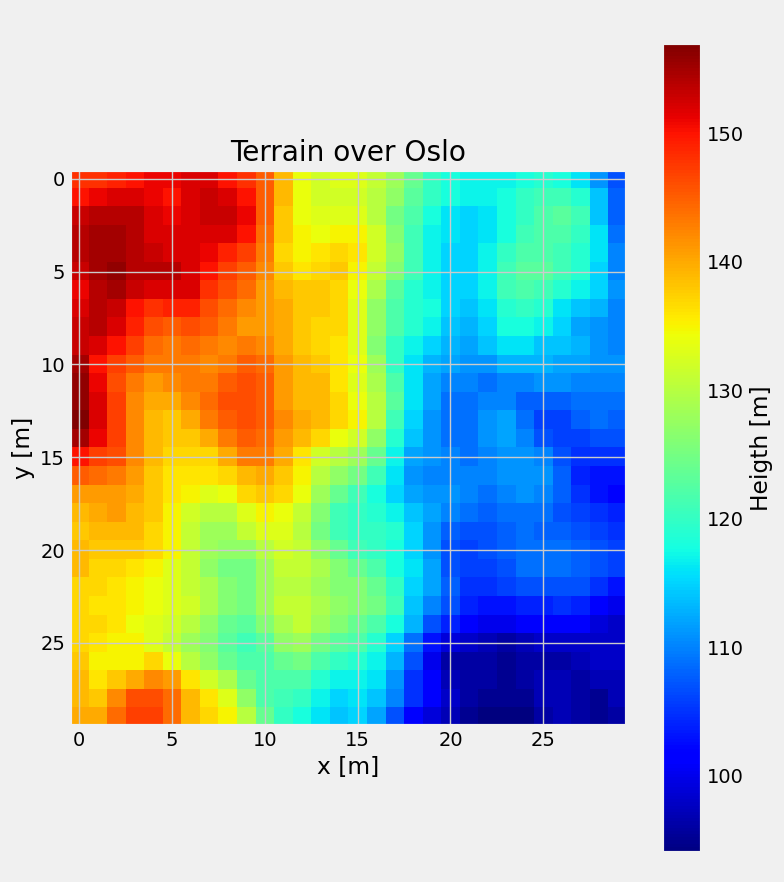
\includegraphics[width=0.5\textwidth]{Figures/terrain_colormap.png}
    \caption{Color map of terrain data used for model fitting. The x and y
        coordinates are latitudinal and longitudinal in meters relative to the upper left
    corner.}  
    \label{fig:terrain_colormap} 
\end{figure}


\begin{table}
    \centering
    \caption{Corner positions of Oslo radar topography data taken in the SRTM mission in the year 2000.}  
    \begin{tabular}{|c|c|}
    	\hline
    	Corner & Position\\
    	\hline
    	NW & Lat 60\degree 00'00"N, Long 10\degree 00'00"E\\
	\hline
	NE & Lat 60\degree 00'00"N, Long 11\degree 00'00"E\\
	\hline
	SE & Lat 59\degree 00'00"N, Long 11\degree 00'00"E\\
	\hline
	SW & Lat 59\degree 00'00"N, Long 10\degree 00'00"E\\
	\hline
    \end{tabular}\label{tab:radar_data} 
\end{table}

\subsection{Error estimation}
%Maybe something about implementation of this
To assess the accuracy of our models we will use the mean squared error
$$
MSE(\boldsymbol{y},\tilde{\boldsymbol{y}}) = \frac{1}{n}
\sum_{i=0}^{n-1}(y_i-\tilde{y}_i)^2,
$$
where n is the number of datapoints. This measures the difference between the model value and the actual value and will be taken from sklearn.metrics. And we will use the score function
$$
R^2(\boldsymbol{y}, \tilde{\boldsymbol{y}}) = 1 - \frac{\sum_{i=0}^{n - 1} (y_i - \tilde{y}_i)^2}{\sum_{i=0}^{n - 1} (y_i - \bar{y})^2},
$$
which is used to score the model and we will take this from sklearn's LinearRegression().fit.score.

\subsection{Linear regression}
\subsubsection{Design matrix} \label{sec:design_matrix} 

Our training data was fitted to polynomials up
to degree 12 in x and y for the Franke function and data, and up to degree 30
for the terrain data. Thus, a design matrix of the form:
\begin{equation*}
    X = 
    \begin{bmatrix}

        1 & x_{0} & y_0 & x_{0}^{2} & x_0 y_0 & y^2 & \dots &y_{0}^{p} \\
        1 & x_{1} & y_1 & x_{1}^{2} & x_1 y_1 & y^2 & \dots &y_{1}^{p} \\
        1 & x_{2} & y_2 & x_{2}^{2} & x_2 y_2 & y^2 & \dots &y_{2}^{p} \\
        \vdots &\vdots &\vdots &\vdots &\vdots & \vdots & \ddots & \vdots \\
        1&x_{n-1} & y_{n-1} & x_{n-1}^2 & x_{n-1} y_{n-1} & y_{n-1}^2 & \dots &y_{n-1}^{p}, 
    \end{bmatrix}
\end{equation*}
was used for OLS-, Ridge- and Lasso regression. To generate our design matrix we used the function
\begin{lstlisting}
FUNCTION create_X(x, y, n)
	X = array(size p, size n)
	FOR i = 1 TO i = p
		q = int((i)*(i+1)/2)
		FOR k = 0 TO k = i
			X[:,q+k] = (x**(i-k))*(y**k)
		ENDFOR
	ENDFOR
	return X
ENDFUNCTION
\end{lstlisting}
This function is based on the lecture notes of Morten Hjorth-Jensen \cite{w35}.
Here p is the polynomial degree and X is the Deign matrix. 
In order to reduce the number of computations, we generated one Design matrix
with number of features corresponding to the maximum polynomial degree $p_{max}
= 12$. This matrix has l features including the intercept given by the
equation: 
\begin{equation}
        \label{eq:l_features} 
        l(p) = int(((p+1)*(p+2)/2))		
\end{equation}
In order to fit the lower order polynomials this matrix was sliced in the
following way
\begin{equation*}
    X_{\text{train}}[:,l(p)].
\end{equation*}

  
% XXX: added y terms to matrix
% XXX: Changed from poly p-1 to p
% %We used the Vandermonde design matrix for a linear regression polynomial fit. No point in having a theory section about this.
% \begin{center}
% $V=
% \begin{bmatrix} 
% 1 & x_{0}&x_{0}^{2}&\dots &x_{0}^{p-1}
% \\1&x_{1}&x_{1}^{2}&\dots &x_{1}^{p-1}
% \\1&x_{2}&x_{2}^{2}&\dots &x_{2}^{p-1}
% \\ \vdots &\vdots &\vdots &\ddots &\vdots \\
% 1&x_{n-1}&ax_{n-1}^{2}&\dots &x_{n-1}^{p-1}
% \end{matrix}
% $
% \end{center}




\subsection{Regression methods} \label{sec:regression_methods}
Since sklearn does not implement the use of psudo-inverse, which is a SVD based
inverse we will write our own regression methods and use numpy's psudo-inverse.
This is because otherwise we get a limitation on the polynomial degree as the
determinant of the Hessian matrix of the training set will go to zero, meaning
that the matrix will be singular and not invertible. We show this in table
\ref{tab:determinants}, where we calculated the determinant of the Hessian matrix with respect to the
training data, with $N_{\text{train }} = 160 $ rows, for different polynomial
degrees (p). 

\begin{table}
    \centering
    \caption{Determinant of $(X^T_{train}X_{train})$ with respect to polynomial
    degree, using N=???????}
    \begin{tabular}{|c|c|}
        \hline
        Polynomial degree & $det(X_{train}^T X_{train})$  \\
        \hline
        1 & 208035.65\\
        \hline
        2 & 891473.68\\
        \hline
        3 & 99.34\\
        \hline
        4 & 7.91$\cdot10^{-10}$ \\
        \hline
        5 & 8.58$\cdot10^{-31}$ \\
        \hline
        6 & 1.92$\cdot10^{-64}$ \\
        \hline
        7 & 1.13$\cdot10^{-113}$ \\
        \hline
        8 & 5.28$\cdot10^{-181}$ \\
        \hline
        9 & 2.21$\cdot10^{-269}$ \\
        \hline
        10 & 0.0 \\
        \hline
        11 & 0.0 \\
        \hline
        12 & 0.0 \\
        \hline
    \end{tabular}\label{tab:determinants}
\end{table}


\subsubsection{OLS}
%%OLS
%How did we implement it
%Why did we implement it
%Did we do any testing
We first tried a simple Ordinary Least Square model for fitting the train data. 
The optimal values for beta (our polynomial coefficient's) with OLS regression $\hat{\bm{\beta}  }_{OLS}$ was
calculated from equation
\eqref{eq:beta_OLS}. We compared our own OLS with Sklearn's method
(sklearn.linear\_model.LinearRegression). For the same training data, without
any re-sampling. Both methods agreed up to polynomial fits of degree nine.
For polynomials of degree larger than 9, the two methods was no longer in
agreement on the Mean Squared Error (see figure \ref{fig:ols_skl_vs_own}). This
probably due to the fact that sklearn's OLS method not uses the pseudo inverse
as discussed in section \ref{sec:regression_methods} 

\begin{figure}[H]
    \centering
    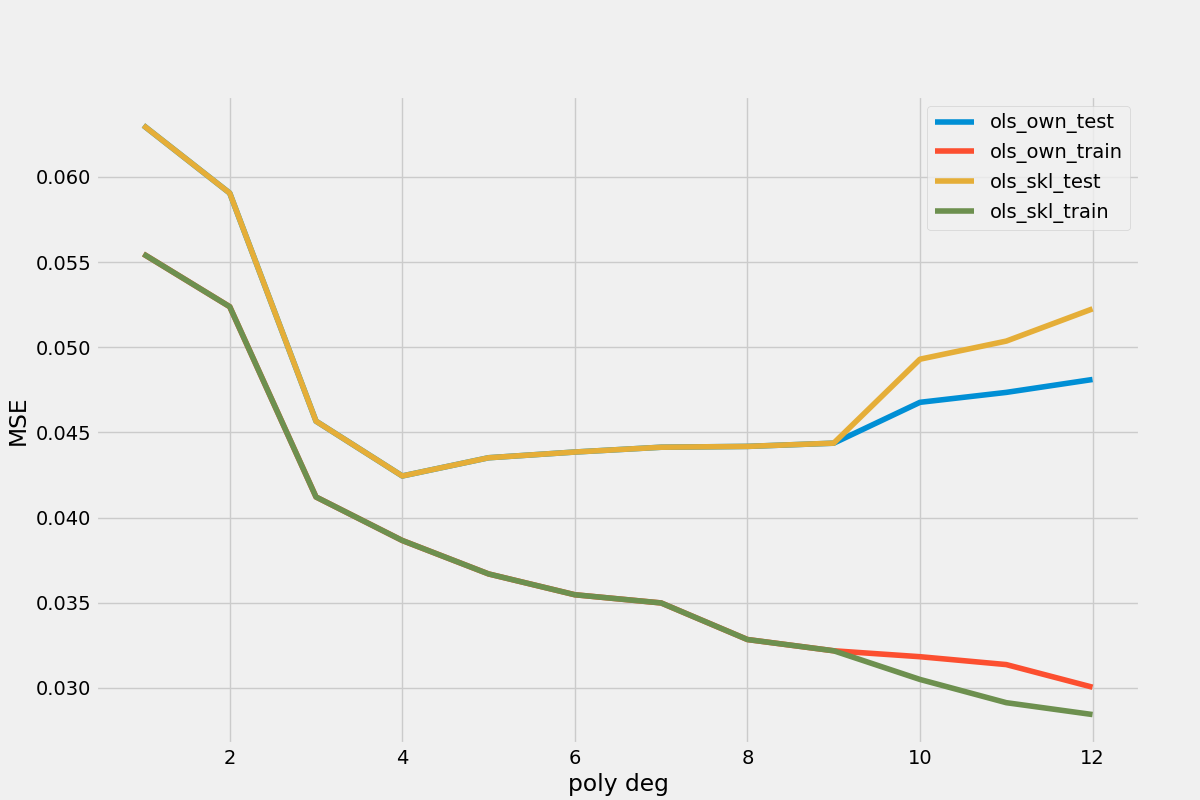
\includegraphics[width=0.5\textwidth]{Figures/test_mse_sklearn_vs_own.png}
    \caption{Comparison MSE produced from our own OLS method and sklearn's,
    predicted on the test and train data obtained from the Franke function. The
training data was used fro finding the optimal model with OLS}  
    \label{fig:ols_skl_vs_own} 
\end{figure}

%%MÅ HA PLOT ELLER LIKNENDE OM MAN SKAL SI DETTE. ELLER DET MÅ VÆRE I RESULTS.

%Skrev noe liknende i avsnitt over
%The solution only exist when $(\bm{X}^T \bm{X})$ is
%invertible. To circumvent this problem we used numpy's pseudo inverse, to invert
%the matrix.


\subsubsection{Ridge}
%%Ridge
%How did we implement it
%Why did we implement it
%Did we do any testing
In the case of Ridge regression we introduced an array of regularization
parameters $\lambda = [10^{-6}, 10^{-5}, \hdots, 10^{1}]$. The optimal values
of beta with ridge regression $\hat{\bm{\beta } } _{Ridge} $ was calculated
from equation \eqref{eq:beta_ridge}. For implementing equation we used numpy.eye as the iidentity matrix. 

\subsubsection{Lasso}
%%Lasso
%How did we implement it
%Why did we implement it
%Did we do any testing
The same regularization parameters as used for Ridge regression was used to find the
optimal values for beta with Lasso regression, $\hat{\bm{\beta } } _{Lasso} $. We did not develop our
own algorithm for Lasso regression. Instead we used the function provided by the
sklearn python module.  

\subsection{Resampling}
%%Bootstrap
???????????
%How did we implement it
%Code snippet
%and what parameter values we used

%%Cross-validation
???????????
%How did we implement it
%Code snippet
%and what parameter values we used


%%%%%%%%%%%%%%%%%%%%%%%%%%%%%%%%%%%%%%%%%%%%%%%%%%%%%%%%%%%%%%%%%%%%%%%%%%%%%%%%%%%%%%%%%%
\section{Results}

%%%%%%%%%%%%%%% Parameters %%%%%%%%%%%%%%%
% n_data = 20 - n_data in x and y: n_tot = 20*20
% test_size = 0.2
% noise = 0.2 - aptitude of normal distributed noise    
% data_dim = 2

%%%%%%%%%%%%%%% Part b %%%%%%%%%%%%%%%
% * Evaluate MSE up to 5.th order fro OLS. 
% * and R2 score
% * blot parameters beta
% * Your code has to include a scaling/centering:
%   XXX: not included, data is already scaled in intervall [-1, 1]

\begin{figure}[H]
    \centering
    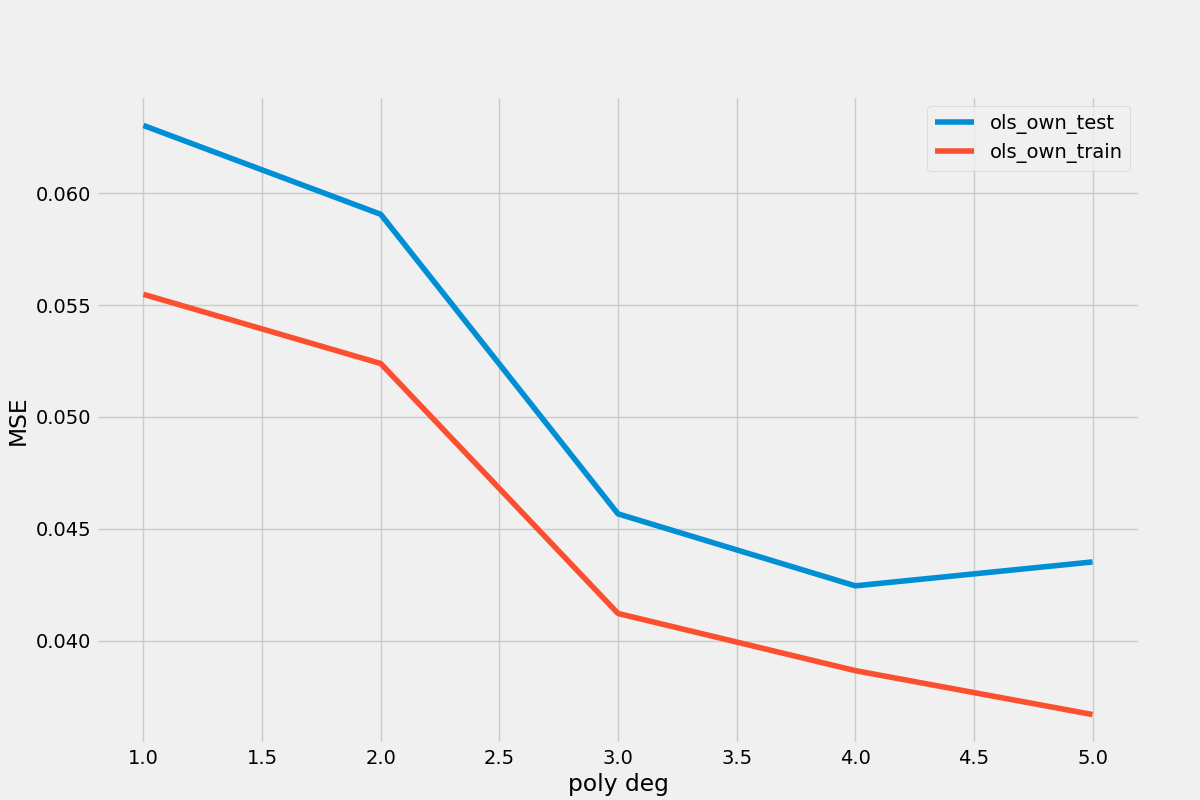
\includegraphics[width=0.8\textwidth]{Figures/b_mse.png}
\end{figure}

\begin{figure}[H]
    \centering
    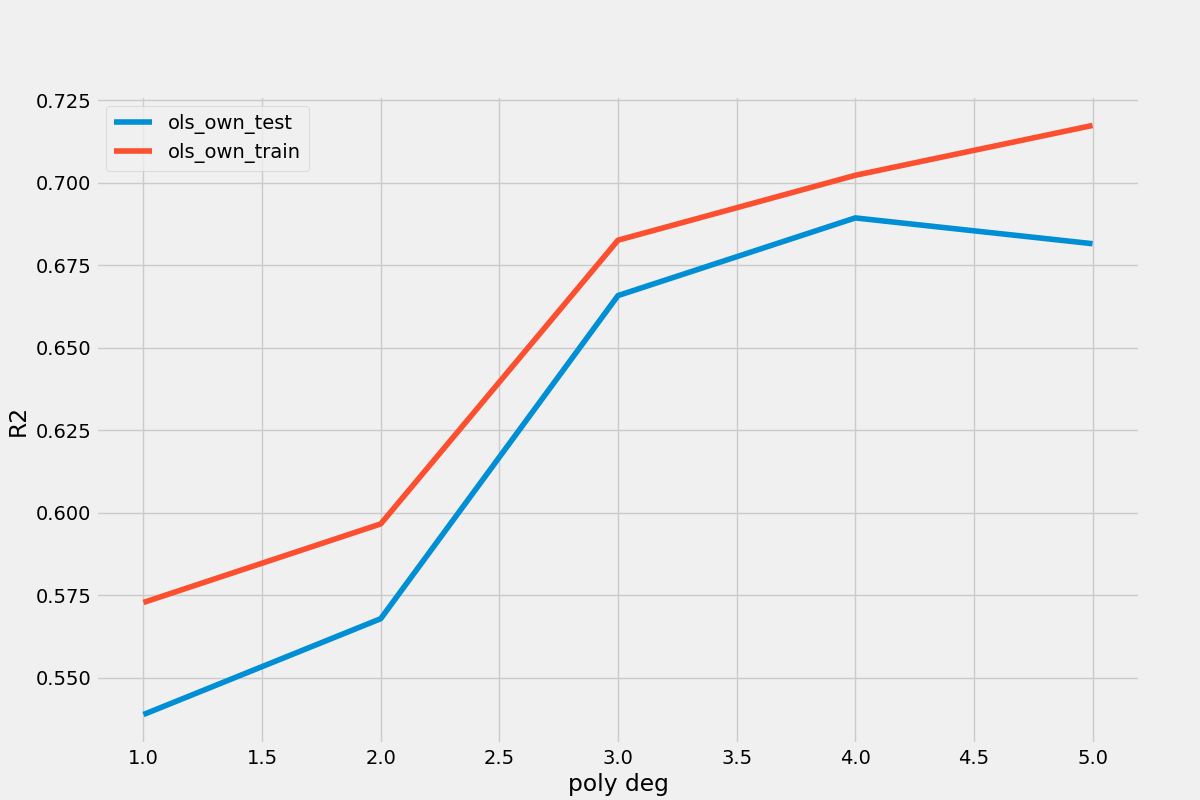
\includegraphics[width=0.8\textwidth]{Figures/b_r2.png}
\end{figure}

% TODO: error bars
\begin{figure}[H]
    \centering
    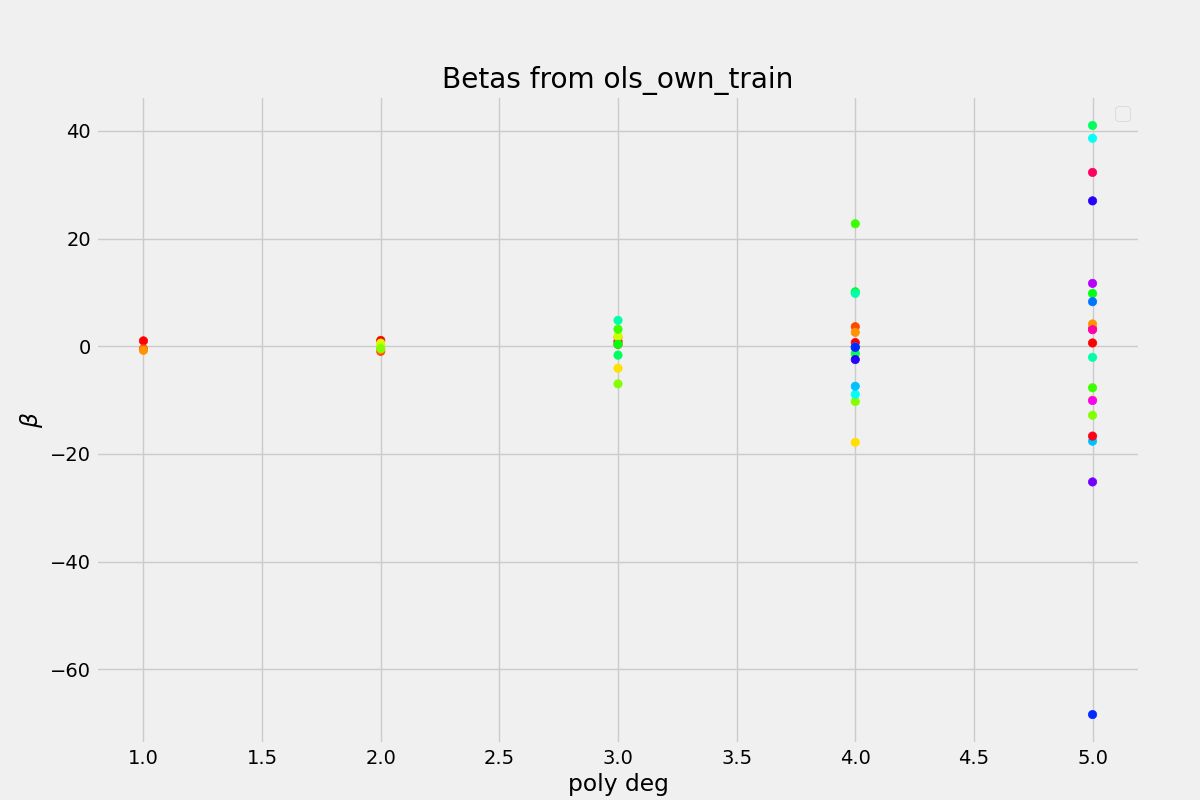
\includegraphics[width=0.8\textwidth]{Figures/b_beta.png}
\end{figure}


%%%%%%%%%%%%%%% Part c  %%%%%%%%%%%%%%%
% * Explain bias, variance, mse terms (theory) and interpretation 
% * Bias variance analysis on franke function
% * discuss in bias variance trade-off in terms of:
%   * model complexity
%   * number of data points
%   * training and test data


\begin{figure}[H]
    \centering
    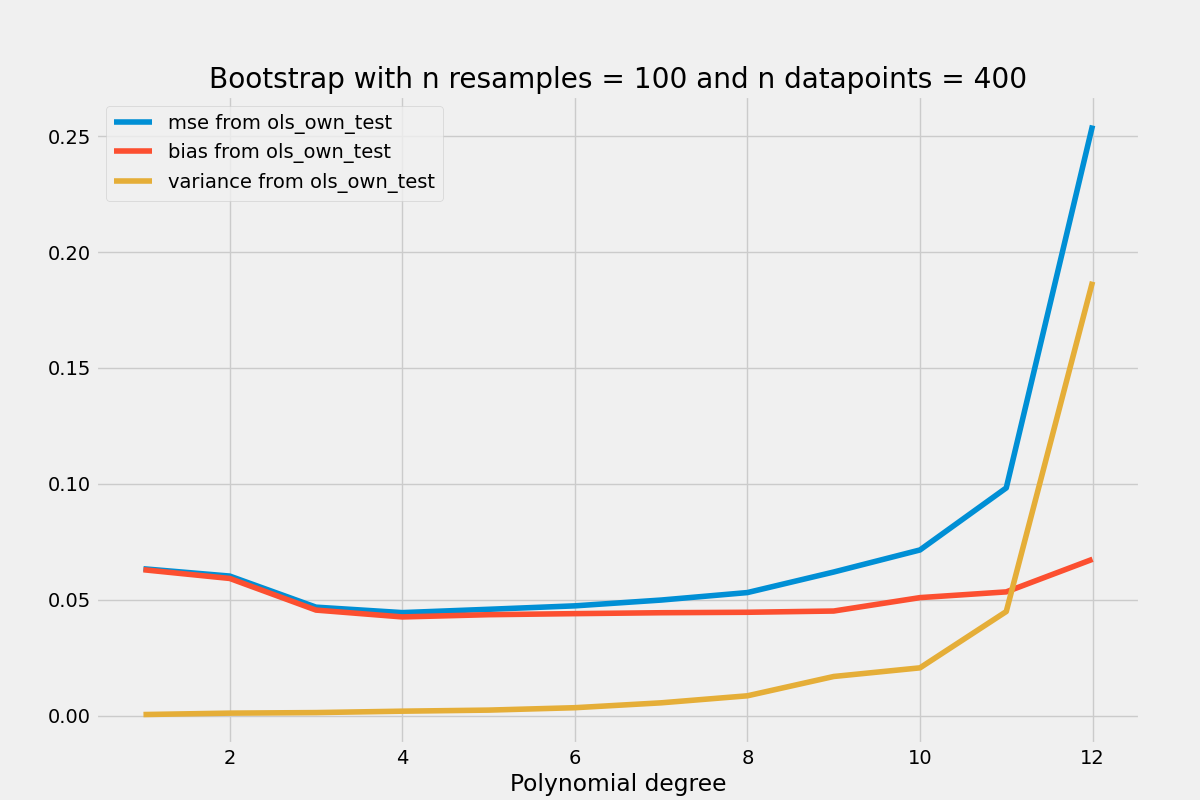
\includegraphics[width=0.8\textwidth]{Figures/c_bootstrap_ols_n_data_400.png}
\end{figure}


\begin{figure}[H]
    \centering
    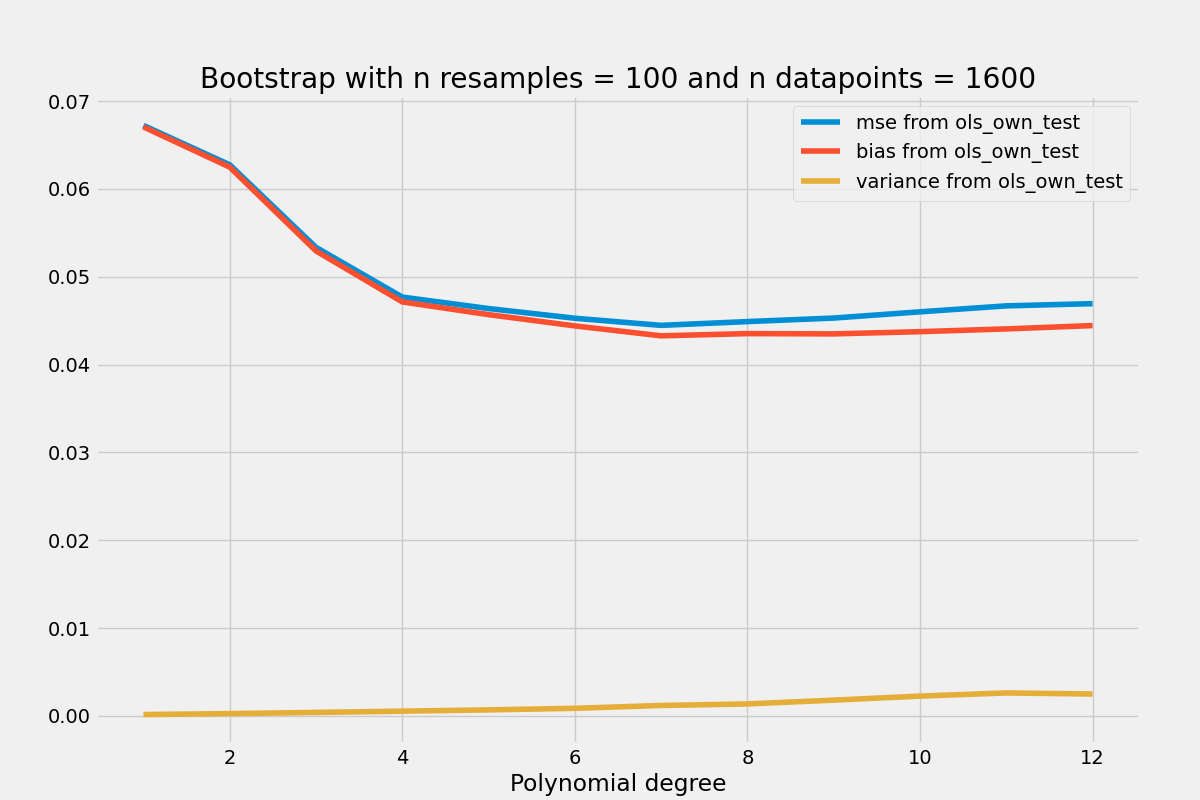
\includegraphics[width=0.8\textwidth]{Figures/c_bootstrap_ols_n_data_1600.png}
\end{figure}

% XXX: Is this expected behaviour?
\begin{figure}[H]
    \centering
    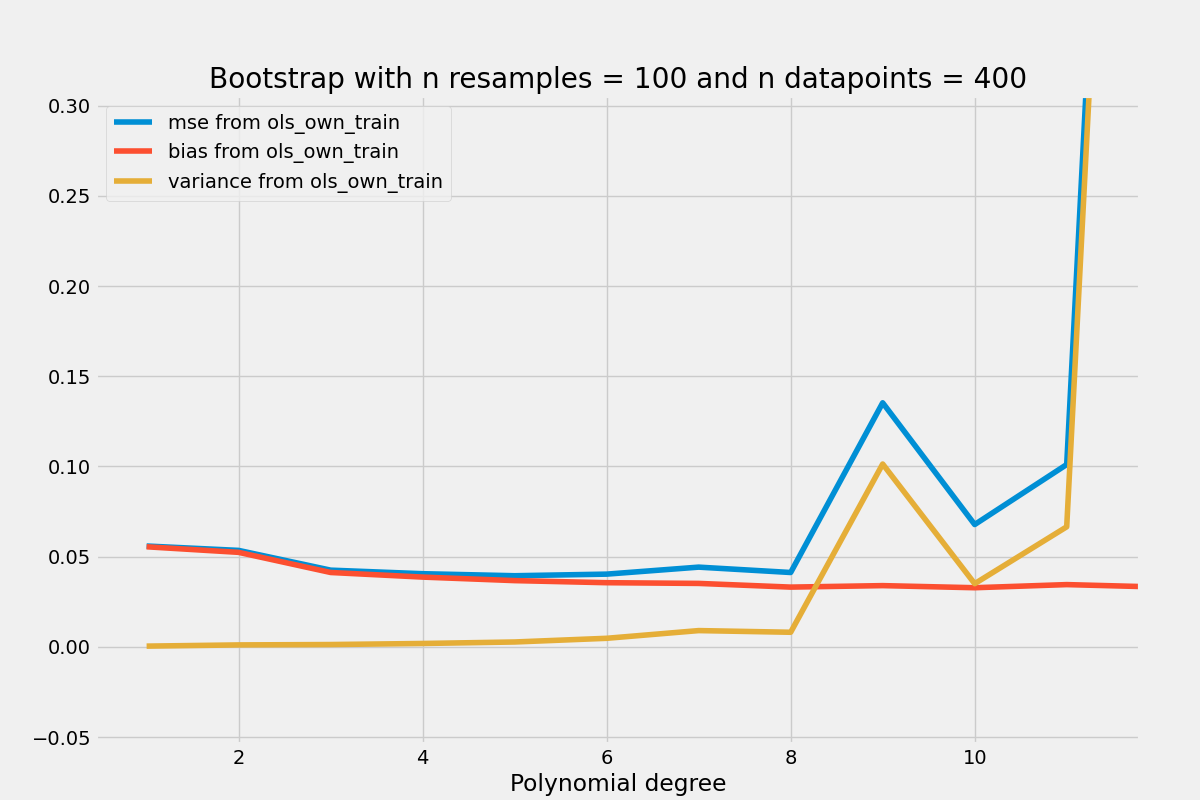
\includegraphics[width=0.8\textwidth]{Figures/c_bootstrap_ols_n_data_400_train_data.png}
\end{figure}

%%%%%%%%%%%%%%% Part d %%%%%%%%%%%%%%%
% Use k-fold and evaluate MEE on test data
% compare with bootstrap
% compare with sklearn

\begin{figure}[H]
    \centering
    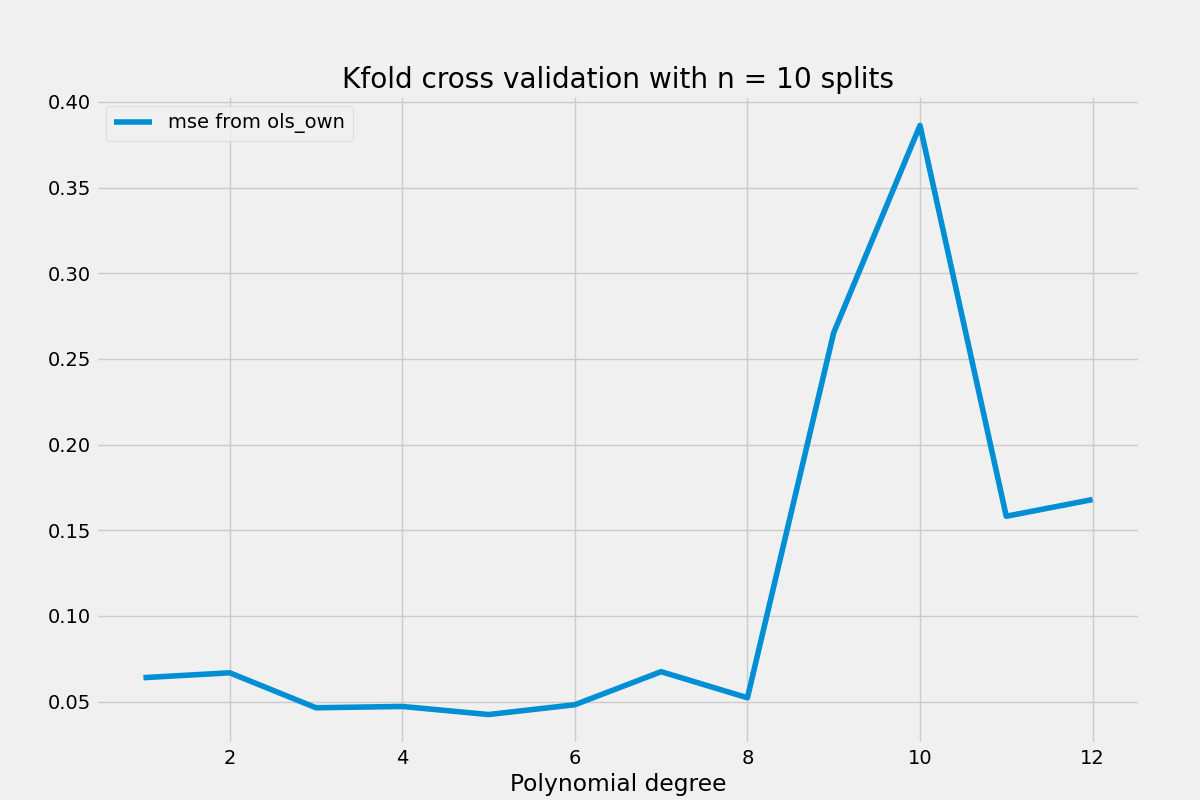
\includegraphics[width=0.8\textwidth]{Figures/d_kfold_ols_n_10.png}
\end{figure}

%%%%%%%%%%%%%%% Part e %%%%%%%%%%%%%%%
% * bootstrap analysis for ridge as in part c
% * and cross validation as in part d 
% * Compare results to those obtained in part b-d
% * study bias variance trade off for different values of lambda 

The minimum MSE from Ridge regression was found for polynomial degree of 6 with
the hyper parameter, $\lambda = 0.001$
\begin{figure}[H]
    \centering
    \caption{ridge}  
    \label{fig:e_ridge} 
    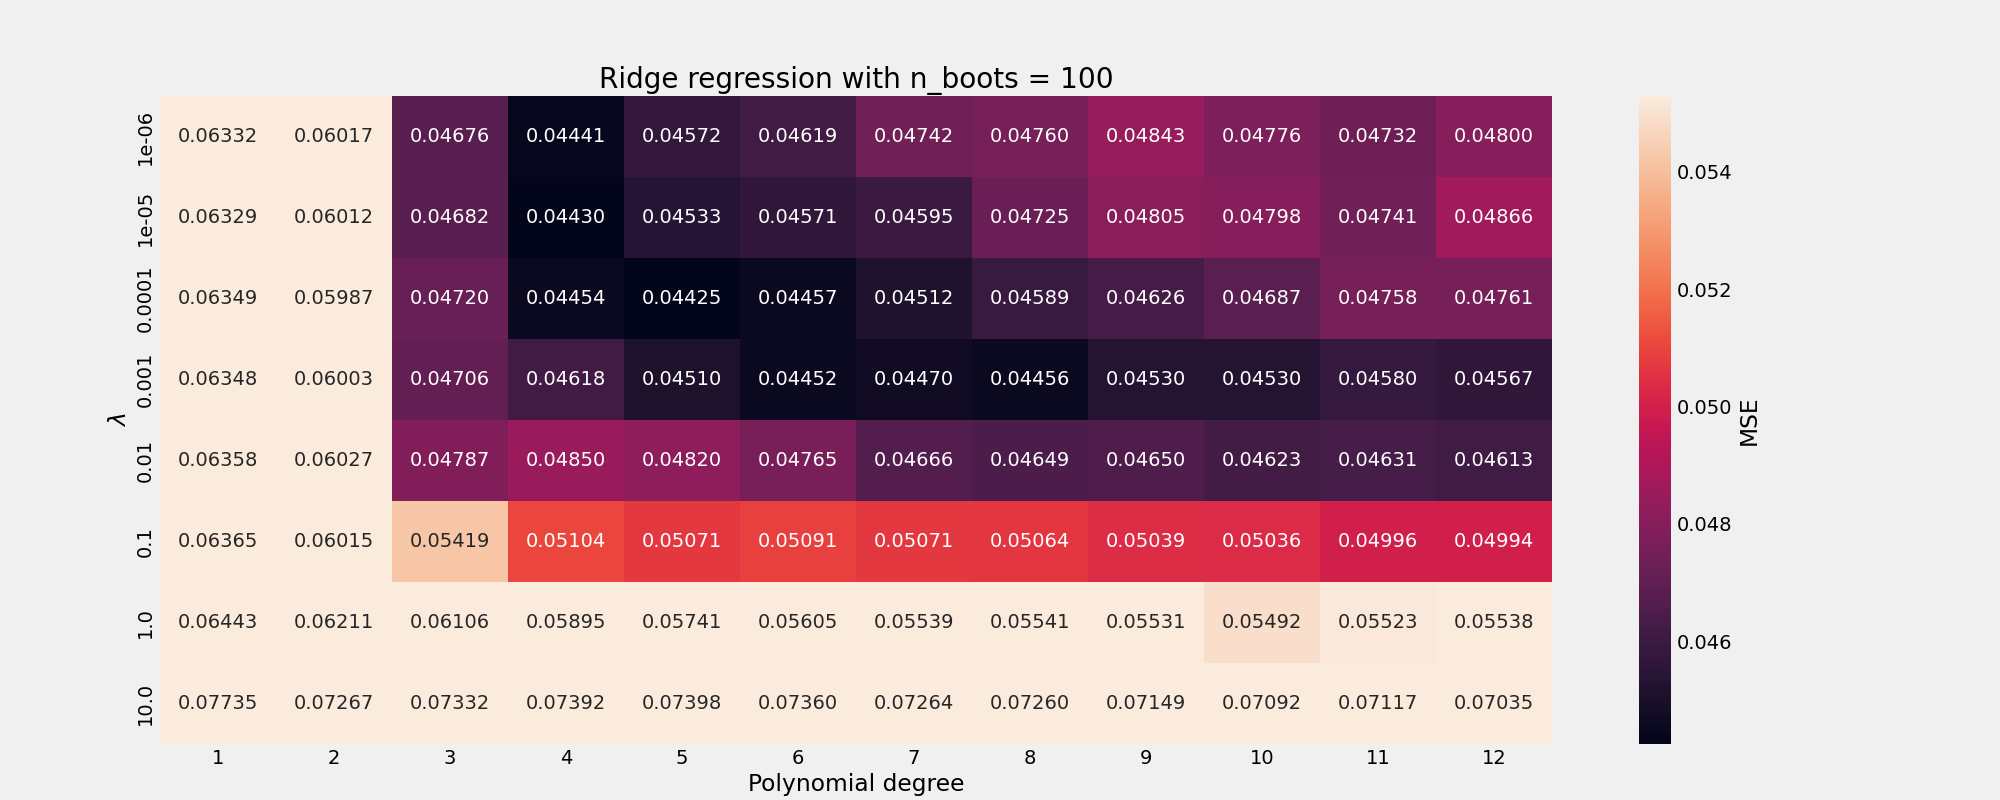
\includegraphics[width=1\textwidth]{Figures/e_ridge_n_boots_100.png}
\end{figure}

\begin{figure}[H]
    \centering
    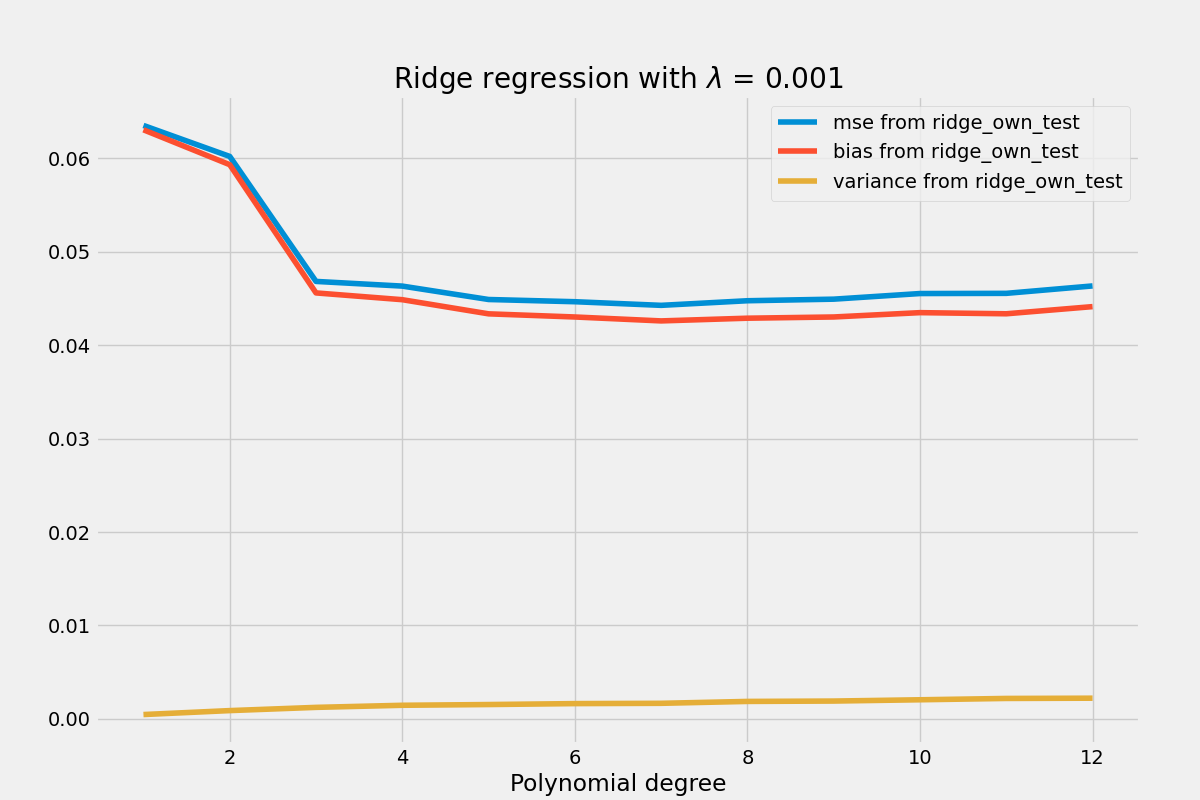
\includegraphics[width=0.8\textwidth]{Figures/e_ridge_bias_variance_lamb_0_001.png}
\end{figure}


\begin{figure}[H]
    \centering
    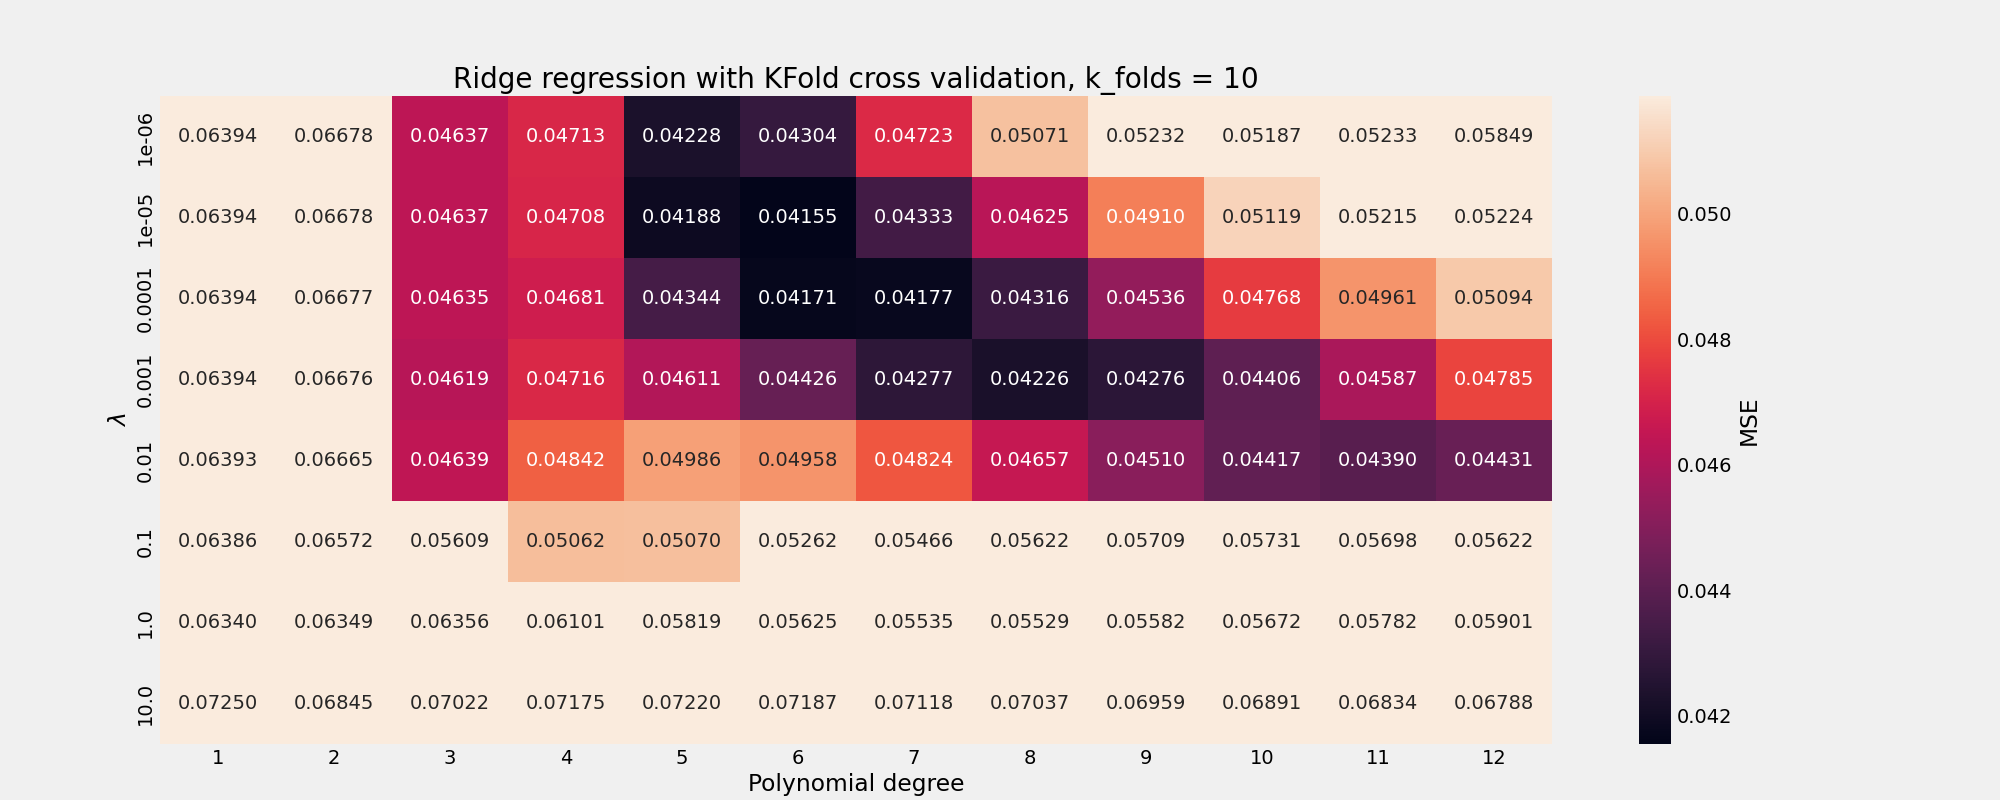
\includegraphics[width=0.8\textwidth]{Figures/e_ridge_kfold_n_10.png}
\end{figure}

%%%%%%%%%%%%%%% Part f %%%%%%%%%%%%%%%
% * Lasso regression
% * give a critical discussion of mse, ridge, lasso
% * Which model fits the data best 
% * bootstrap bias variance analysis of lasso
% * MSE analysis with kfold


\begin{figure}[H]
    \centering
    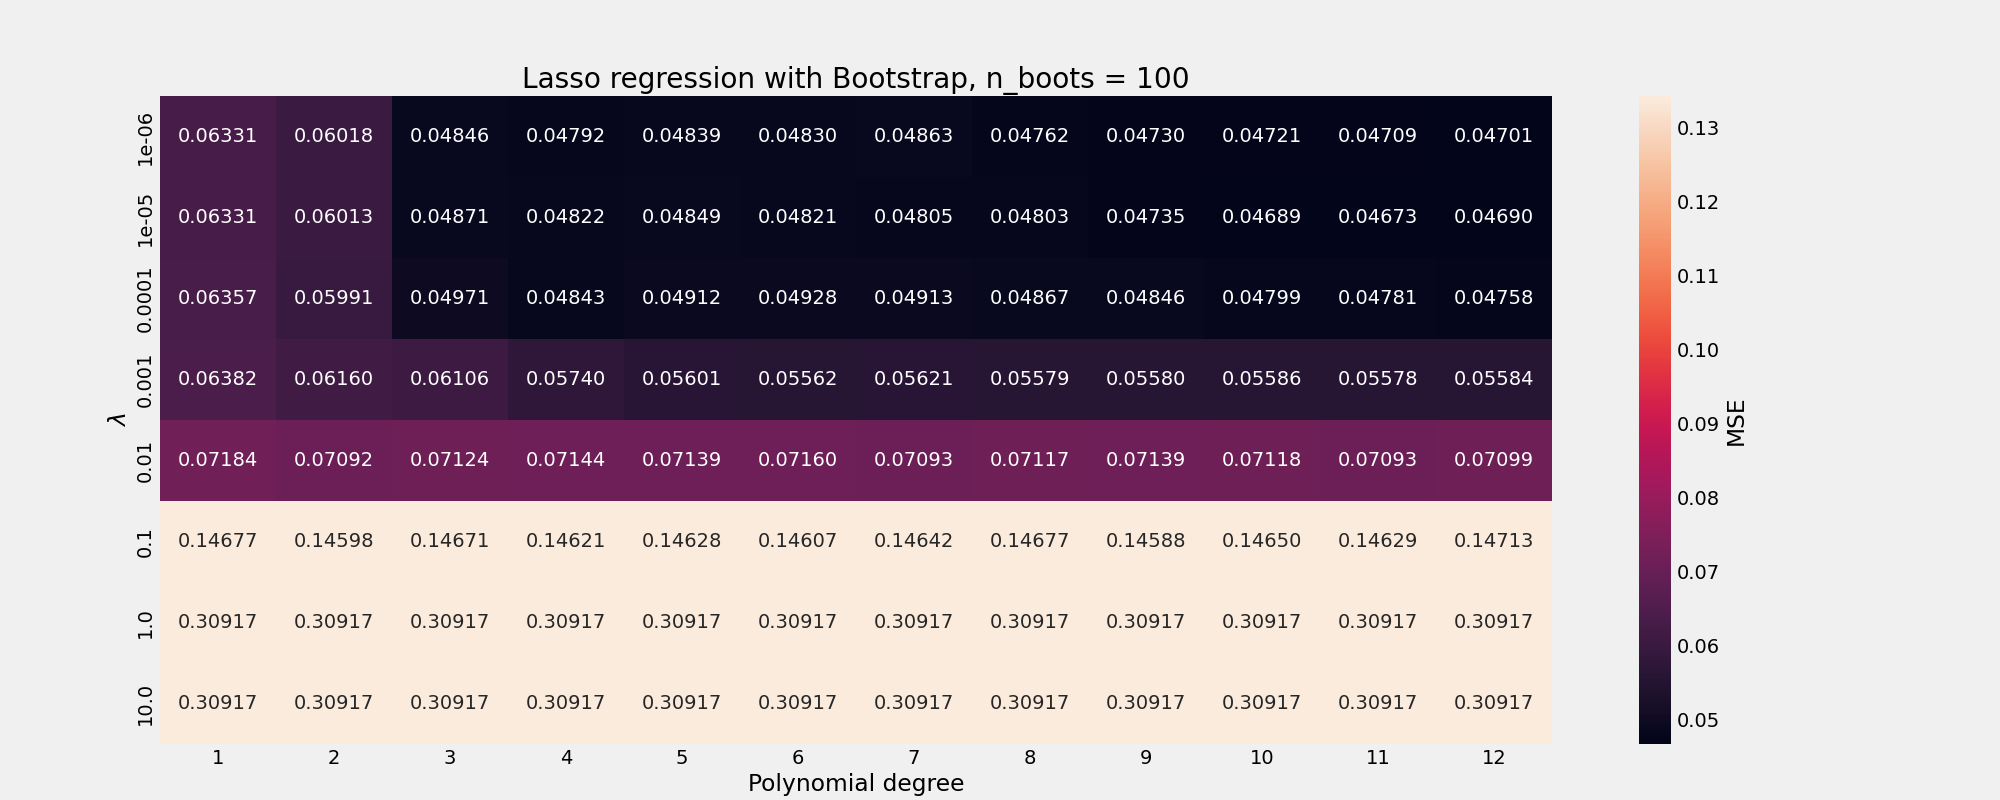
\includegraphics[width=0.8\textwidth]{Figures/f_lasso_bootstrap_n_100.png}
\end{figure}

\begin{figure}[H]
    \centering
    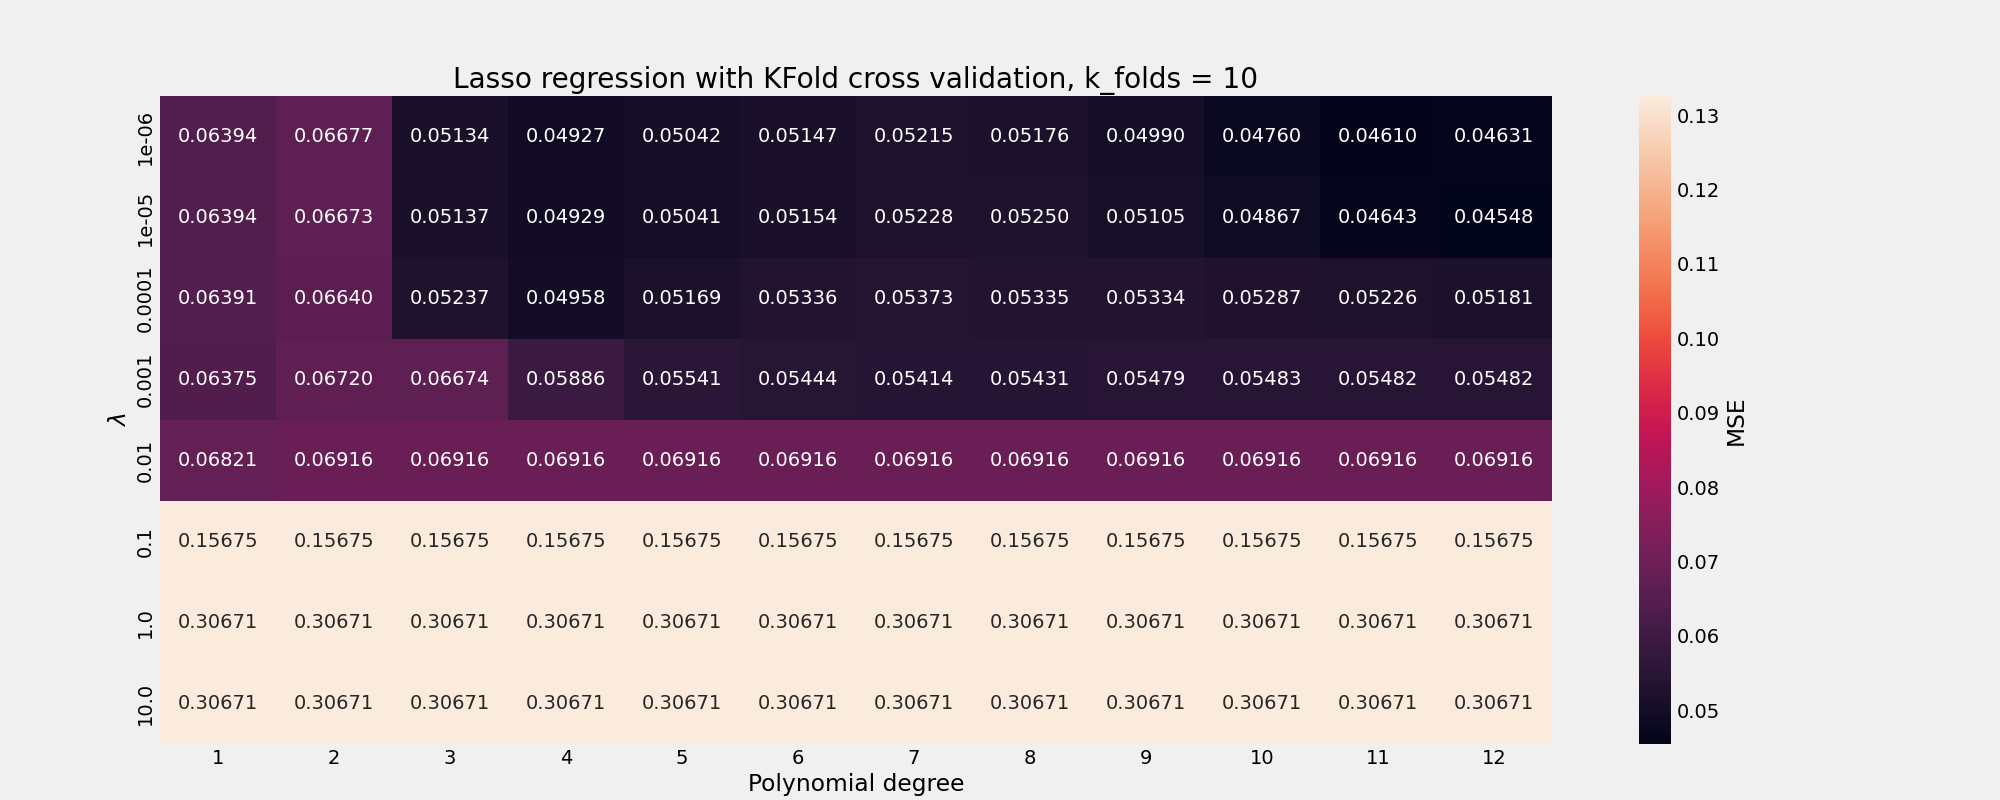
\includegraphics[width=0.8\textwidth]{Figures/f_lasso_kfold_n_10.png}
\end{figure}



% TODO: comparison of MSE for all methods
 

$R^2$ and MSE plot of OLS, Ridge and lasso

%%%%%%%%%%%%%%%%%%%%%%%%%%%%%%%%%%%%%%%%%%%%%%%%%%%%%%%%%%%%%%%%%%%%%%%%%%%%%%%%%%%%%%%%%%
\section{Discussion}


%%%%%%%%%%%%%%%%%%%%%%%%%%%%%%%%%%%%%%%%%%%%%%%%%%%%%%%%%%%%%%%%%%%%%%%%%%%%%%%%%%%%%%%%%%
\section{Conclusion}



We found that using the Lasso and Ridge methods over the OLS on Franke data did not have much benefits on the MSE. But for the terrain data we got a much better with fit with the regularization parameter. This could be because the Franke function is a smooth and easy function to fit and the terrain data can have a much more complex shape. We also found that for the Franke function bootstrapping and k-fold resampling decreased the total error of the model up to certain polynomial degrees where the variance got exponentially higher because of overfitting. This is because when working with a smaller dataset, overfitting will happen sooner. For the Lasso and Ridge method we found that the $\beta$-parameters was smaller with Ridge than Lasso. This can be seen from the cost-function of each of the methods as the Lasso has the 1-norm and Ridge has the 2-norm. This makes Ridge regularize the $\beta$-parameters more.

\appendix
\section{Expectation values and variances for ordinary least squares}\label{app:ols_expactation_variance}
%Some equations copied from lecture notes but this part is finished I think. Maybe should write it a bit better since it's a lot of we get that, we then, we we we
We use that the dependent variable
$$
y_i = y(x_i) = \tilde{y}_i + \epsilon_i = \mathbf X_{i*}\boldsymbol{\beta} + \epsilon_i,
$$

to get the expectation value



$$
\mathbb{E}[y_i] = \mathbb{E}[\mathbf X_{i*}\boldsymbol{\beta} + \epsilon_i] = \mathbb{E}[\mathbf X_{i*}\boldsymbol{\beta}] + \mathbb{E}[\epsilon_i].
$$

We now use that $\epsilon_i$ is a normal distributed error, meaning that $\mathbb{E}[\epsilon_i]=0$. And we assume that $\mathbf X_{i*}\boldsymbol{\beta}$ are not stocastic variables, giving $\mathbb{E}[\mathbf X_{i*}\boldsymbol{\beta}]=\mathbf X_{i*}\boldsymbol{\beta}$. Then the expectaion value is

\begin{equation}\label{eq:expectation_yi}
\mathbb{E}[y_i] = \mathbf X_{i*}\boldsymbol{\beta}.
\end{equation}

We then calculate the variance


\begin{align*}
\mbox{Var}[y_i] =& \mathbb{E}[y_i^2] - (\mathbb{E}[y_i])^2 = \mathbb{E}[(\mathbf X_{i*}\boldsymbol{\beta} + \epsilon_i)^2]- (\mathbf X_{i*}\boldsymbol{\beta})^2
\\
\ =& \mathbb{E}[(\mathbf X_{i*}\boldsymbol{\beta})^2+2\epsilon_i \mathbf X_{i*}\boldsymbol{\beta}+\epsilon_i^2]-(\mathbf X_{i*}\boldsymbol{\beta})^2
\\
\ =& \mathbb{E}[(\mathbf X_{i*}\boldsymbol{\beta})^2] + \mathbb{E}[2\epsilon_i \mathbf X_{i*}\boldsymbol{\beta}] + \mathbb{E}[\epsilon_i^2]-(\mathbf X_{i*}\boldsymbol{\beta})^2
\\
\ =& (\mathbf X_{i*}\boldsymbol{\beta})^2 + 2\mathbf X_{i*}\boldsymbol{\beta}\mathbb{E}[\epsilon_i ] + \mathbb{E}[\epsilon_i^2]-(\mathbf X_{i*}\boldsymbol{\beta})^2
\\
\ =& 2\mathbf X_{i*}\boldsymbol{\beta}\mathbb{E}[\epsilon_i ] + \mathbb{E}[\epsilon_i^2],
\end{align*}


where we have taken the non stochastic variables out of the expectation value. We again use that the expectation value of a normal distributed variable is $\mathbb{E}[\epsilon_i ]=0$, and see that the variance of this variable is
$$
\mbox{Var}[\epsilon_i]=\mathbb{E}[\epsilon_i^2 ]-(\mathbb{E}[\epsilon_i ])^2=\mathbb{E}[\epsilon_i^2 ]=\sigma^2.
$$
Using this we get
\begin{equation}\label{eq:var_yi}
\mbox{Var}[y_i] = \sigma^2.
\end{equation}



The optimal parameter $\hat{\boldsymbol{\beta}}$ for ordinary least squares is given by

$$
\hat{\boldsymbol\beta}=(\mathbf{X}^T\mathbf{X})^{-1}\mathbf{X}^T\mathbf{y}
$$


We then calculate the expectation value of the optimal parameter

$$
\mathbb{E}(\boldsymbol{\hat{\beta}}) = \mathbb{E}[ (\mathbf{X}^{\top} \mathbf{X})^{-1}\mathbf{X}^{T} \mathbf{y}]=(\mathbf{X}^{T} \mathbf{X})^{-1}\mathbf{X}^{T} \mathbb{E}[ \mathbf{y}],
$$
where we assume that $\mathbf{X}$ is non stochastic. Using the expectation value from equation (\ref{eq:expectation_yi}) on vector form we get

\begin{equation}\label{eq:expectation_beta_app}
\mathbb{E}(\boldsymbol{\hat{\beta}}) = (\mathbf{X}^{T} \mathbf{X})^{-1} \mathbf{X}^{T}\mathbf{X}\boldsymbol{\beta}=\boldsymbol{\beta}.
\end{equation}

We then calculate the variance of the optimal parameter

\begin{align*}
\mbox{Var}(\boldsymbol{\hat{\beta}}) 
&= \mathbb{E}[(\boldsymbol{\hat\beta} - \mathbb{E}[\boldsymbol{\hat\beta}])^2 ]
\\
&= \mathbb{E}[((\mathbf{X}^T\mathbf{X})^{-1}\mathbf{X}^T\mathbf{y}-\boldsymbol\beta)^2] 
\\
&= \mathbb{E} \{ [(\mathbf{X}^{T} \mathbf{X})^{-1} \, \mathbf{X}^{T} \mathbf{y} - \boldsymbol{\beta}] \, [(\mathbf{X}^{T} \mathbf{X})^{-1} \, \mathbf{X}^{T} \mathbf{y} - \boldsymbol{\beta}]^{T} \}
\\
&=  \mathbb{E} \{ [(\mathbf{X}^{T} \mathbf{X})^{-1} \, \mathbf{X}^{T} \mathbf{y}] \, [(\mathbf{X}^{T} \mathbf{X})^{-1} \, \mathbf{X}^{T} \mathbf{y}]^{T} \} - \boldsymbol{\beta} \, \boldsymbol{\beta}^{T}
\\
&=  \mathbb{E} \{ (\mathbf{X}^{T} \mathbf{X})^{-1} \, \mathbf{X}^{T} \mathbf{y} \, \mathbf{y}^{T} \, \mathbf{X} \, (\mathbf{X}^{T} \mathbf{X})^{-1}  \} - \boldsymbol{\beta} \, \boldsymbol{\beta}^{T}
\\
&= (\mathbf{X}^{T} \mathbf{X})^{-1} \, \mathbf{X}^{T} \, \mathbb{E} \{ \mathbf{y} \, \mathbf{y}^{T} \} \, \mathbf{X} \, (\mathbf{X}^{T} \mathbf{X})^{-1} - \boldsymbol{\beta} \, \boldsymbol{\beta}^{T}
\\
&= (\mathbf{X}^{T} \mathbf{X})^{-1} \, \mathbf{X}^{T} \, \{ \mathbf{X} \, \boldsymbol{\beta} \, \boldsymbol{\beta}^{T} \,  \mathbf{X}^{T} + \sigma^2 \} \, \mathbf{X} \, (\mathbf{X}^{T} \mathbf{X})^{-1} - \boldsymbol{\beta} \, \boldsymbol{\beta}^{T}
\\
&= (\mathbf{X}^T \mathbf{X})^{-1} \, \mathbf{X}^T \, \mathbf{X} \, \boldsymbol{\beta} \, \boldsymbol{\beta}^T \,  \mathbf{X}^T \, \mathbf{X} \, (\mathbf{X}^T  \mathbf{X})^{-1} +  \, \, \sigma^2 \, (\mathbf{X}^T \mathbf{X})^{-1} \, \mathbf{X}^T  \, \mathbf{X} \, (\mathbf{X}^T \mathbf{X})^{-1} - \boldsymbol{\beta} \boldsymbol{\beta}^T
\\
&= \boldsymbol{\beta} \, \boldsymbol{\beta}^{T}  + \sigma^2 \, (\mathbf{X}^{T} \mathbf{X})^{-1} - \boldsymbol{\beta} \, \boldsymbol{\beta}^{T}
 =  \sigma^2 \, (\mathbf{X}^{T} \mathbf{X})^{-1},
\end{align*}

\begin{equation}\label{eq:var_beta_app}
\mbox{Var}(\boldsymbol{\hat{\beta}})  = \sigma^2 \, (\mathbf{X}^{T} \mathbf{X})^{-1}.
\end{equation}



\end{document}
